% ----------------------------------------------------------------------
\subsection{\pretest}
\label{ss:pretest}

\subsubsection{Purpose}

The \pretest is meant to put the module into an operational state in preparation for more specific tests.
The basic operation of the \roc is checked and some of the default \dac settings are tested.
The \pretest is made up of several subtests, each of which is discussed in turn.

\subsubsection{Methodology}

In the {\tt ProgramRoc} subtest, the ``programmability'' of the \roc is tested.
The value of the total current drawn by the analog amplifiers in all the PUCs (\iana) is measured.
This is done first with the nominal value of \vana, and then again with \vana set to zero.
The difference in \iana from these two measurements should be non-zero,
signifying that \vana is actually being applied to the \roc.
This implies the \roc is capable of receiving commands to alter \dac values, i.e. it is programmable.
The output of this subtest is shown in Figure~\ref{fig:pretest_programROC}.
\\\\
The {\tt SetVana} subtest sets the \vana~\dac so that the total current drawn (\iana) meets a target value (default is 24 mA).
\vana is iteratively adjusted from its default value until it comes within 0.25 mA of the target 
or until 10 iterations have been performed.  The output is shown in Figures~\ref{fig:pretest_Iana} and~\ref{fig:pretest_VanaSettings}.
%\\\\
% Note: as of 9-11-15, the timing test isn't run as part of the fulltest
%The {\tt SetTimings} test \textcolor{red}{FIXME – talk to Doug}
\\\\
The {\tt SetVthrCompCalDel} subtest optimizes the values of the \vthrcomp and \caldel~\dacs.
A sample pixel is chosen from within each \roc with the {\tt
  FindWorkingPixel} function for this test and is assumed to be representative of normal pixel performance.
A scan is performed over \vthrcomp and \caldel to determine which combinations of them put the pixel into an operational state.
At each point in the 256 $\times$ 256 value parameter space,
a number of calibration pulses (default is 5) are sent to the PUC of the chosen pixel.
The number of hits successfully recorded by the pixel is then calculated,
and the results are displayed in the 2D plane of \vthrcomp vs. \caldel 
in what is referred to as a ``tornado plot'' (they looked more like tornados with the older, analog \roc).
Figure~\ref{fig:pretest_pretestVthrCompCalDel_c12_r22} shows a tornado plot.
The red region corresponds to 100\% efficiency \textendash\xspace 
the operational region for the PUC with respect to \vthrcomp and \caldel.
Recall that \vthrcomp is inversely related to the minimum pulse height required to fire the comparator.
The region of \vthrcomp $>$ 150 has zero efficiency because
the threshold of the comparator is so low that the pixel is constantly firing on electronic noise,
and when the calibration pulse is injected,
the pixel is already in an unresponsive state waiting to be read out.
By default \vthrcomp is set 50 DACs higher than the lower edge of the operating plateau,
and \caldel is set halfway between the left and right edges of the
plateau at the chosen \vthrcomp value. Alternatively, the working
point can be set at a point below the higher edge of the operating
plateau by specifying a negative {\tt DeltaVthrComp} value.
The black dot centered within the white square denotes the chosen working point for these two parameters.
Figure~\ref{fig:pretest_pretestCalDel} shows the values of \caldel chosen by the test.

\subsubsection{Output}

\begin{figure}[!htp]
\centering
\begin{minipage}{0.45\textwidth}
  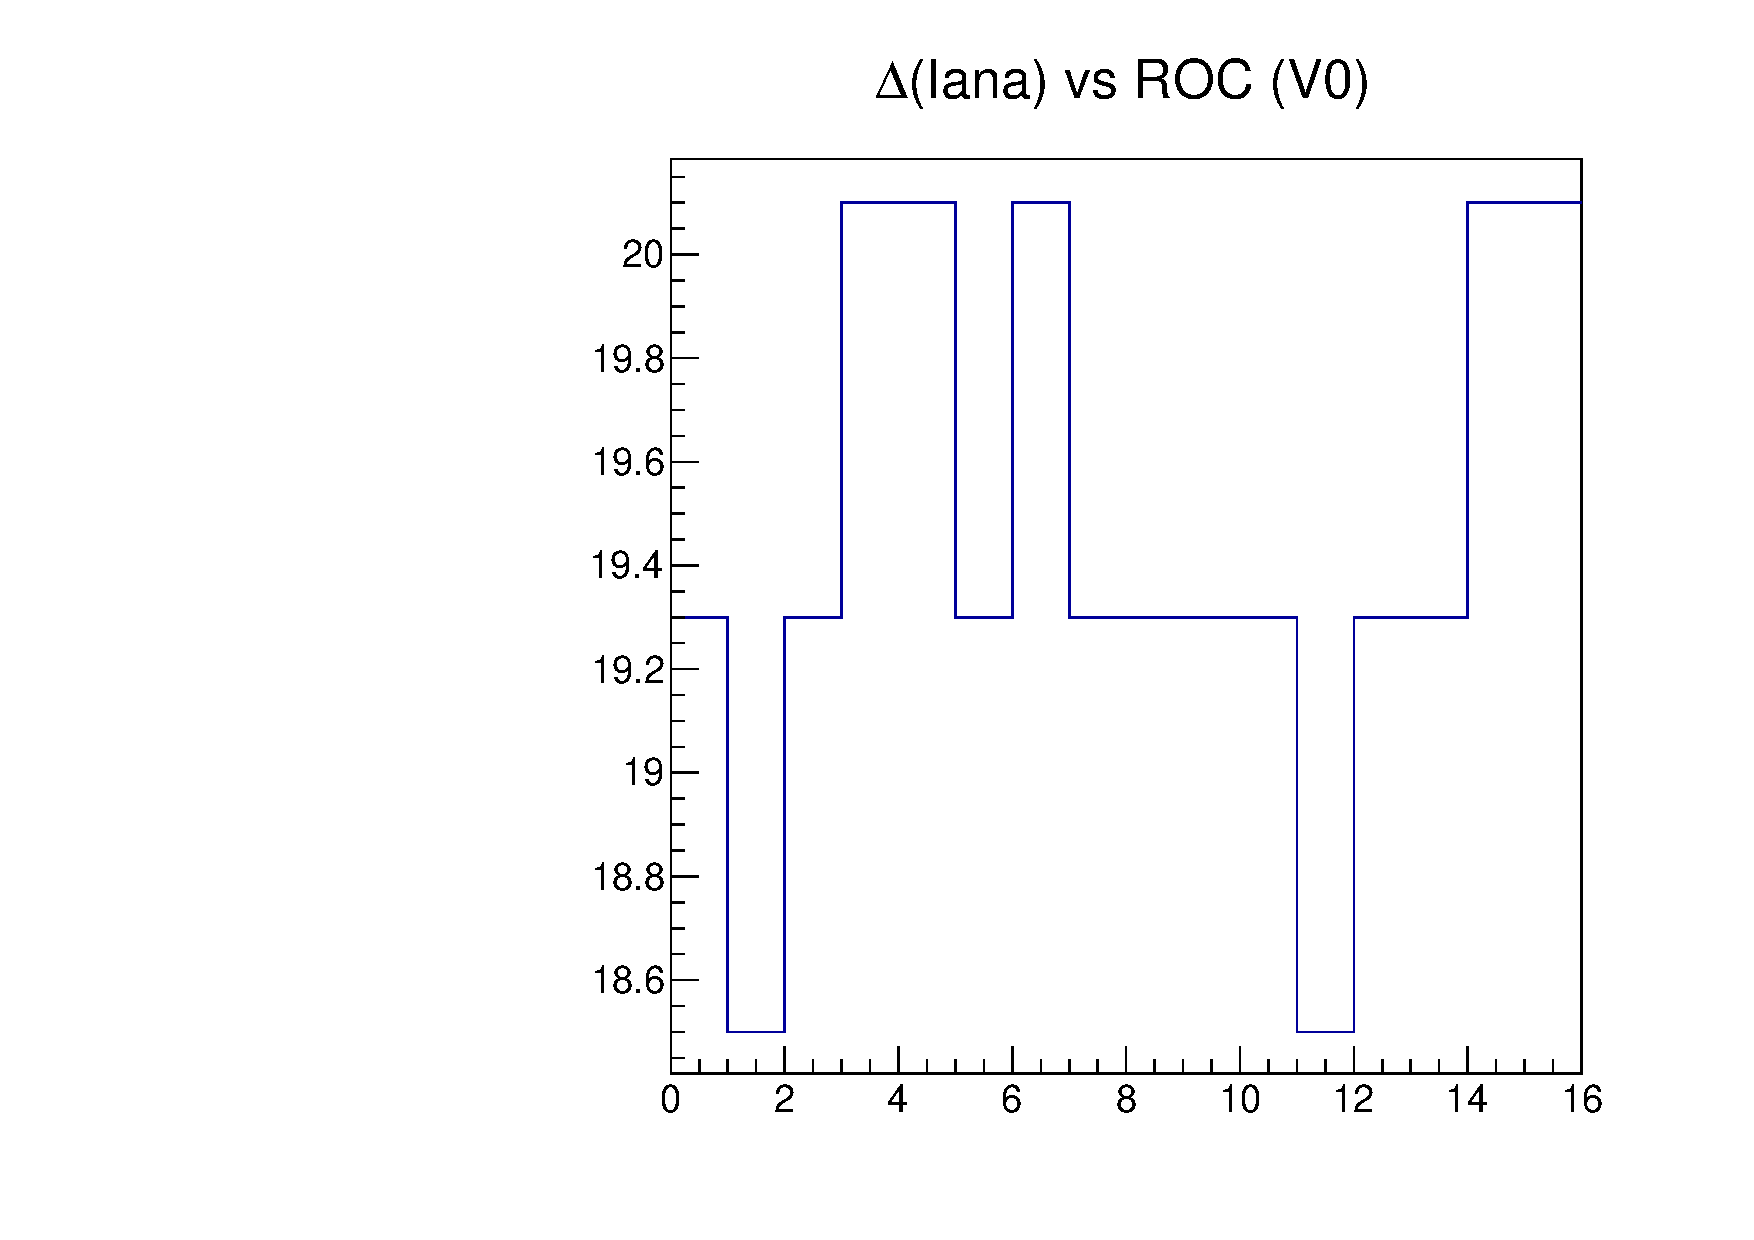
\includegraphics[width=1.0\textwidth]{figures/pretest_programROC.pdf}
  \caption{Created by the {\tt ProgramRoc} subtest. 
    Plotted is the difference in \iana for cases of \vana on/off, as a function of \roc number.
    Values for programmable \rocs are non-zero. Note the
    ordinate zero-suppression.}
  \label{fig:pretest_programROC}
\end{minipage}
\hspace{0.3cm}
\begin{minipage}{0.45\textwidth}
  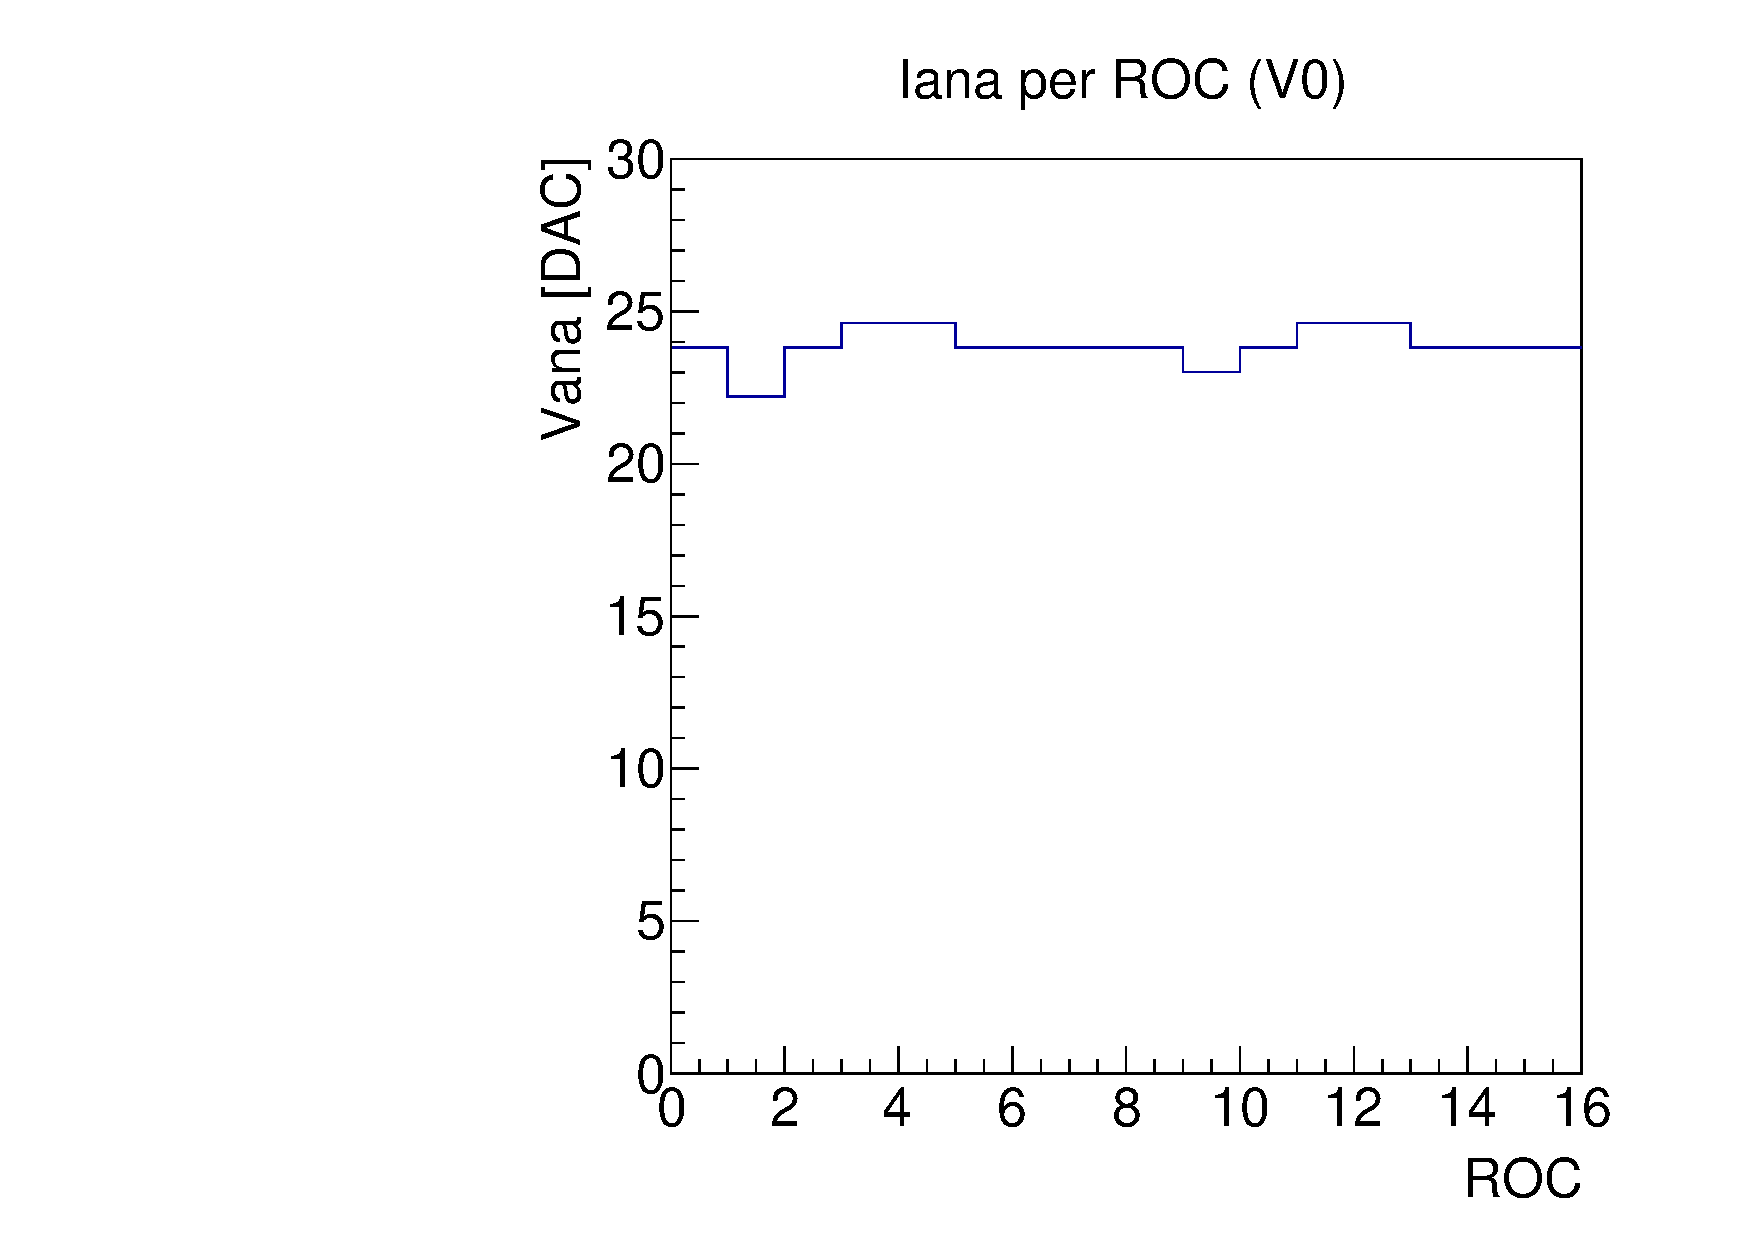
\includegraphics[width=1.0\textwidth]{figures/pretest_Iana.pdf}
  \caption{Created by the {\tt SetVana} subtest.  
    Plotted are the final values of \iana, as a function of \roc number.
    The default target value for \iana is 24 mA.}
  \label{fig:pretest_Iana}
\end{minipage}
\end{figure}

\begin{figure}[!htp]
\centering
\begin{minipage}{0.45\textwidth}
  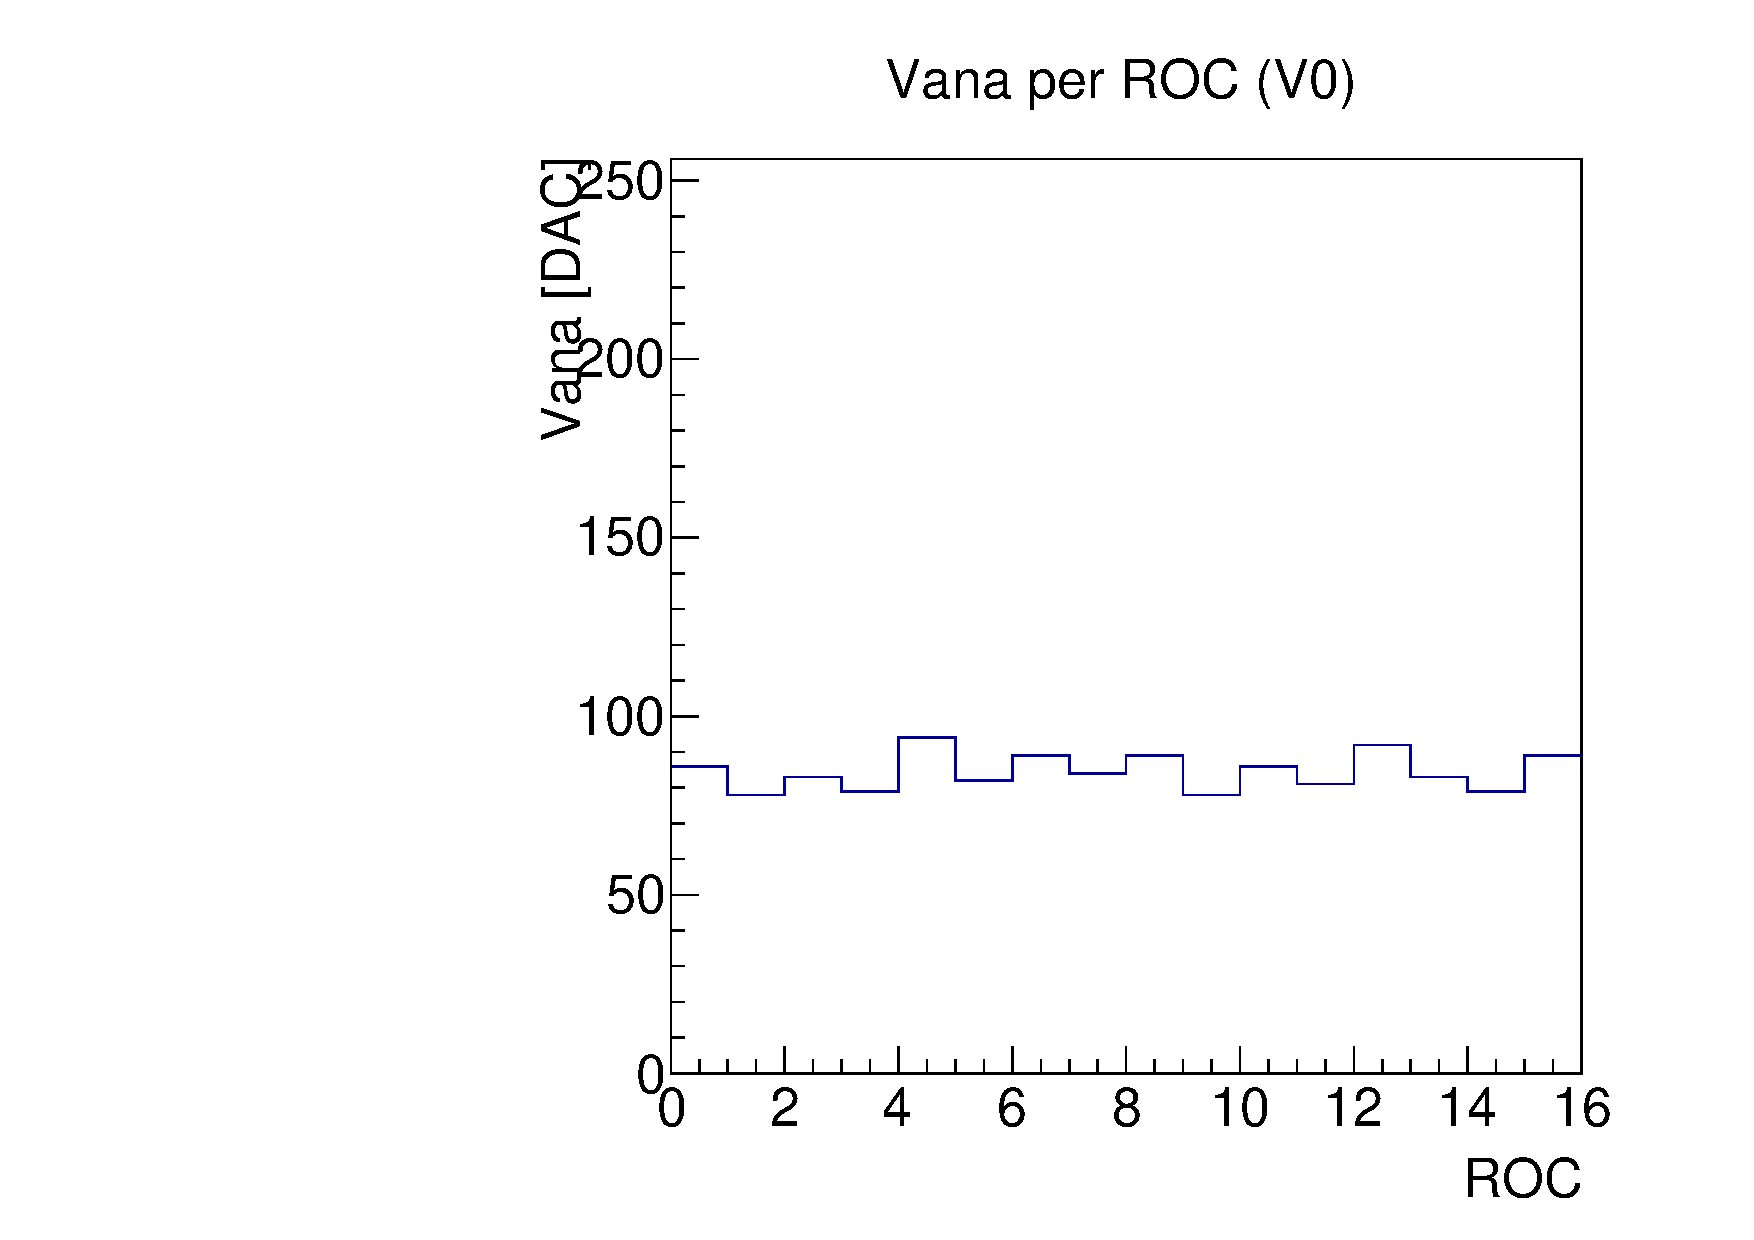
\includegraphics[width=1.0\textwidth]{figures/pretest_VanaSettings.pdf}
  \caption{Created by the {\tt SetVana} subtest.  
    Plotted are the optimized values of \vana, as a function of \roc number.
    For the default \iana target of 24 mA, \vana is roughly 80 DAC units.}
  \label{fig:pretest_VanaSettings}
\end{minipage}
\hspace{0.3cm}
\begin{minipage}{0.45\textwidth}
  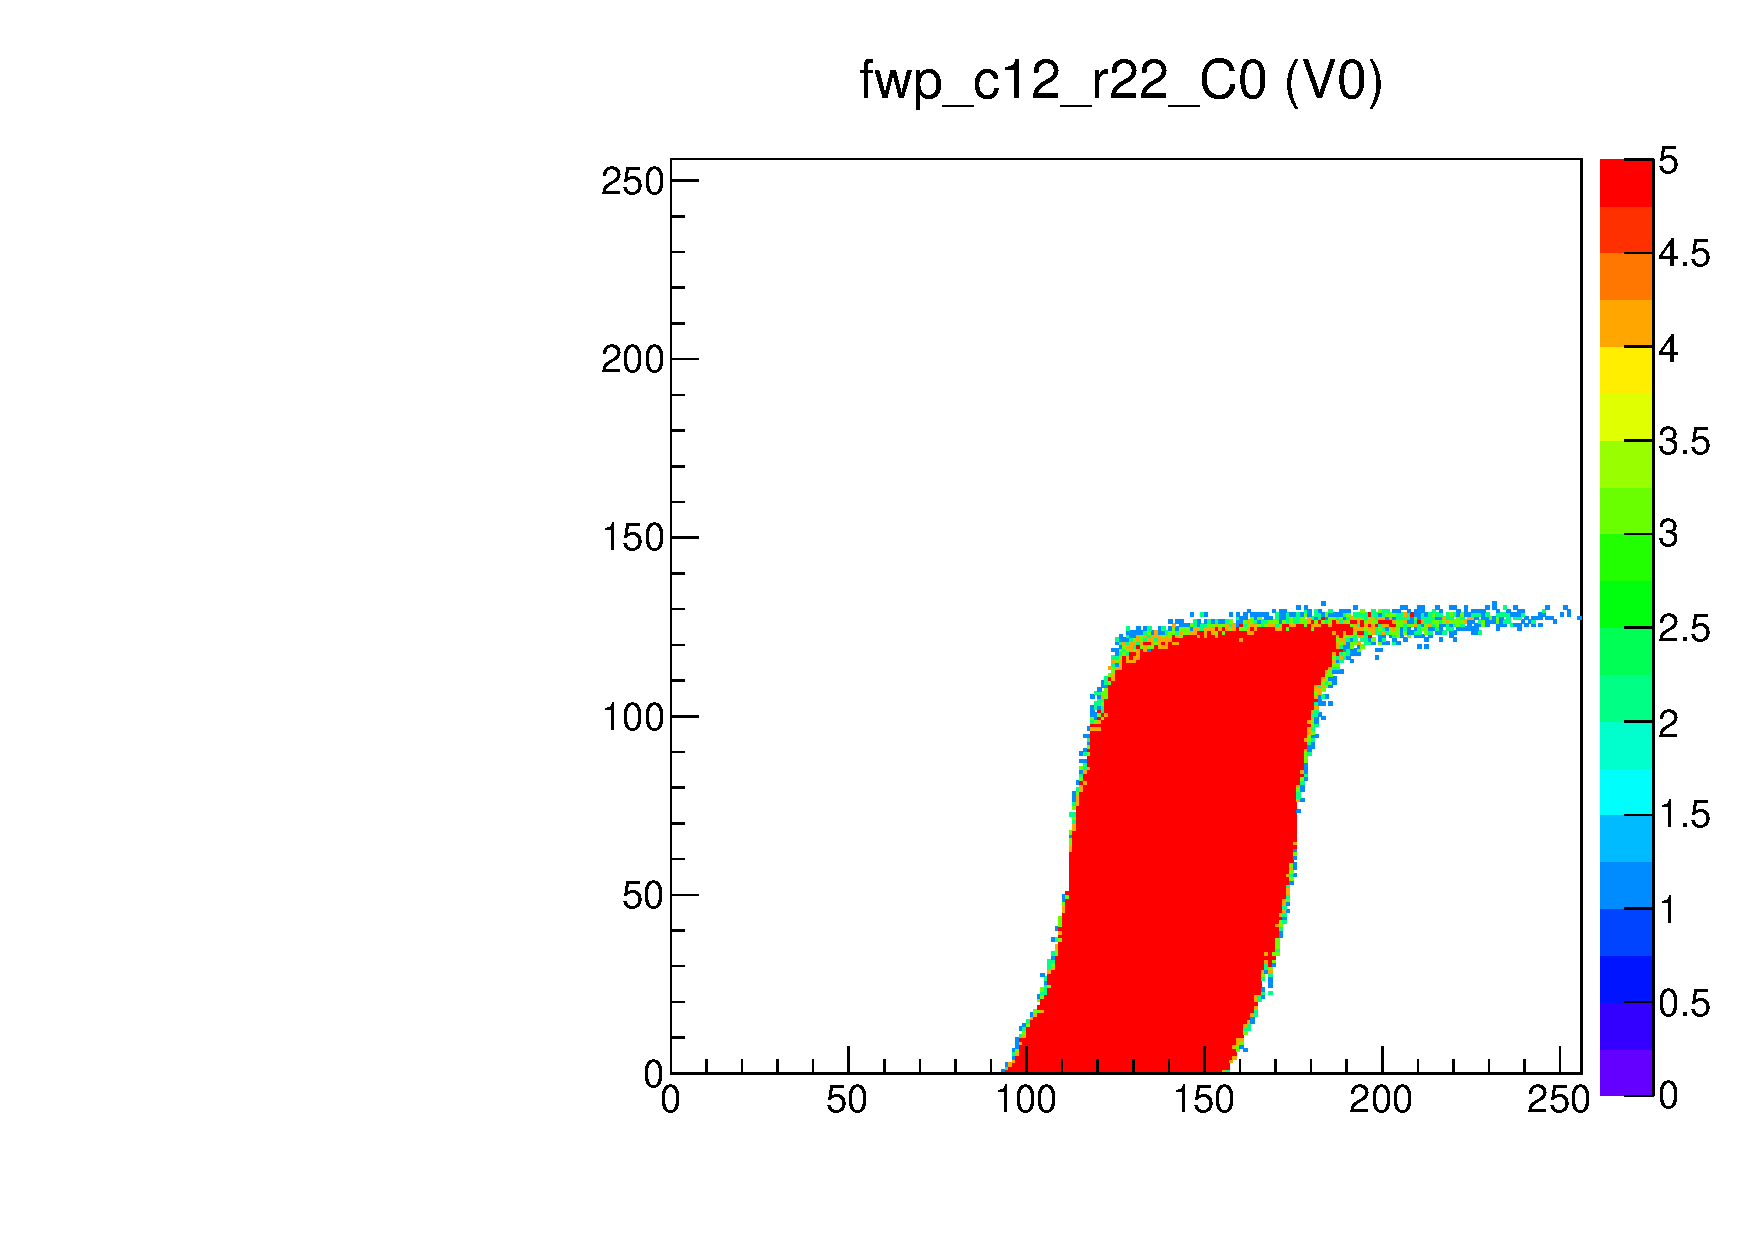
\includegraphics[width=1.0\textwidth]{figures/pretest_fwp_c12_r22.pdf}
  \caption{Created by the {\tt FindWorkingPixel} subtest.
  Similar to Figure~\ref{fig:pretest_pretestVthrCompCalDel_c12_r22},
  but not presetting \vcal.}
  \label{fig:pretest_fwp_c12_r22}
\end{minipage}
\end{figure}

\begin{figure}[!htp]
\centering
\begin{minipage}{0.45\textwidth}
  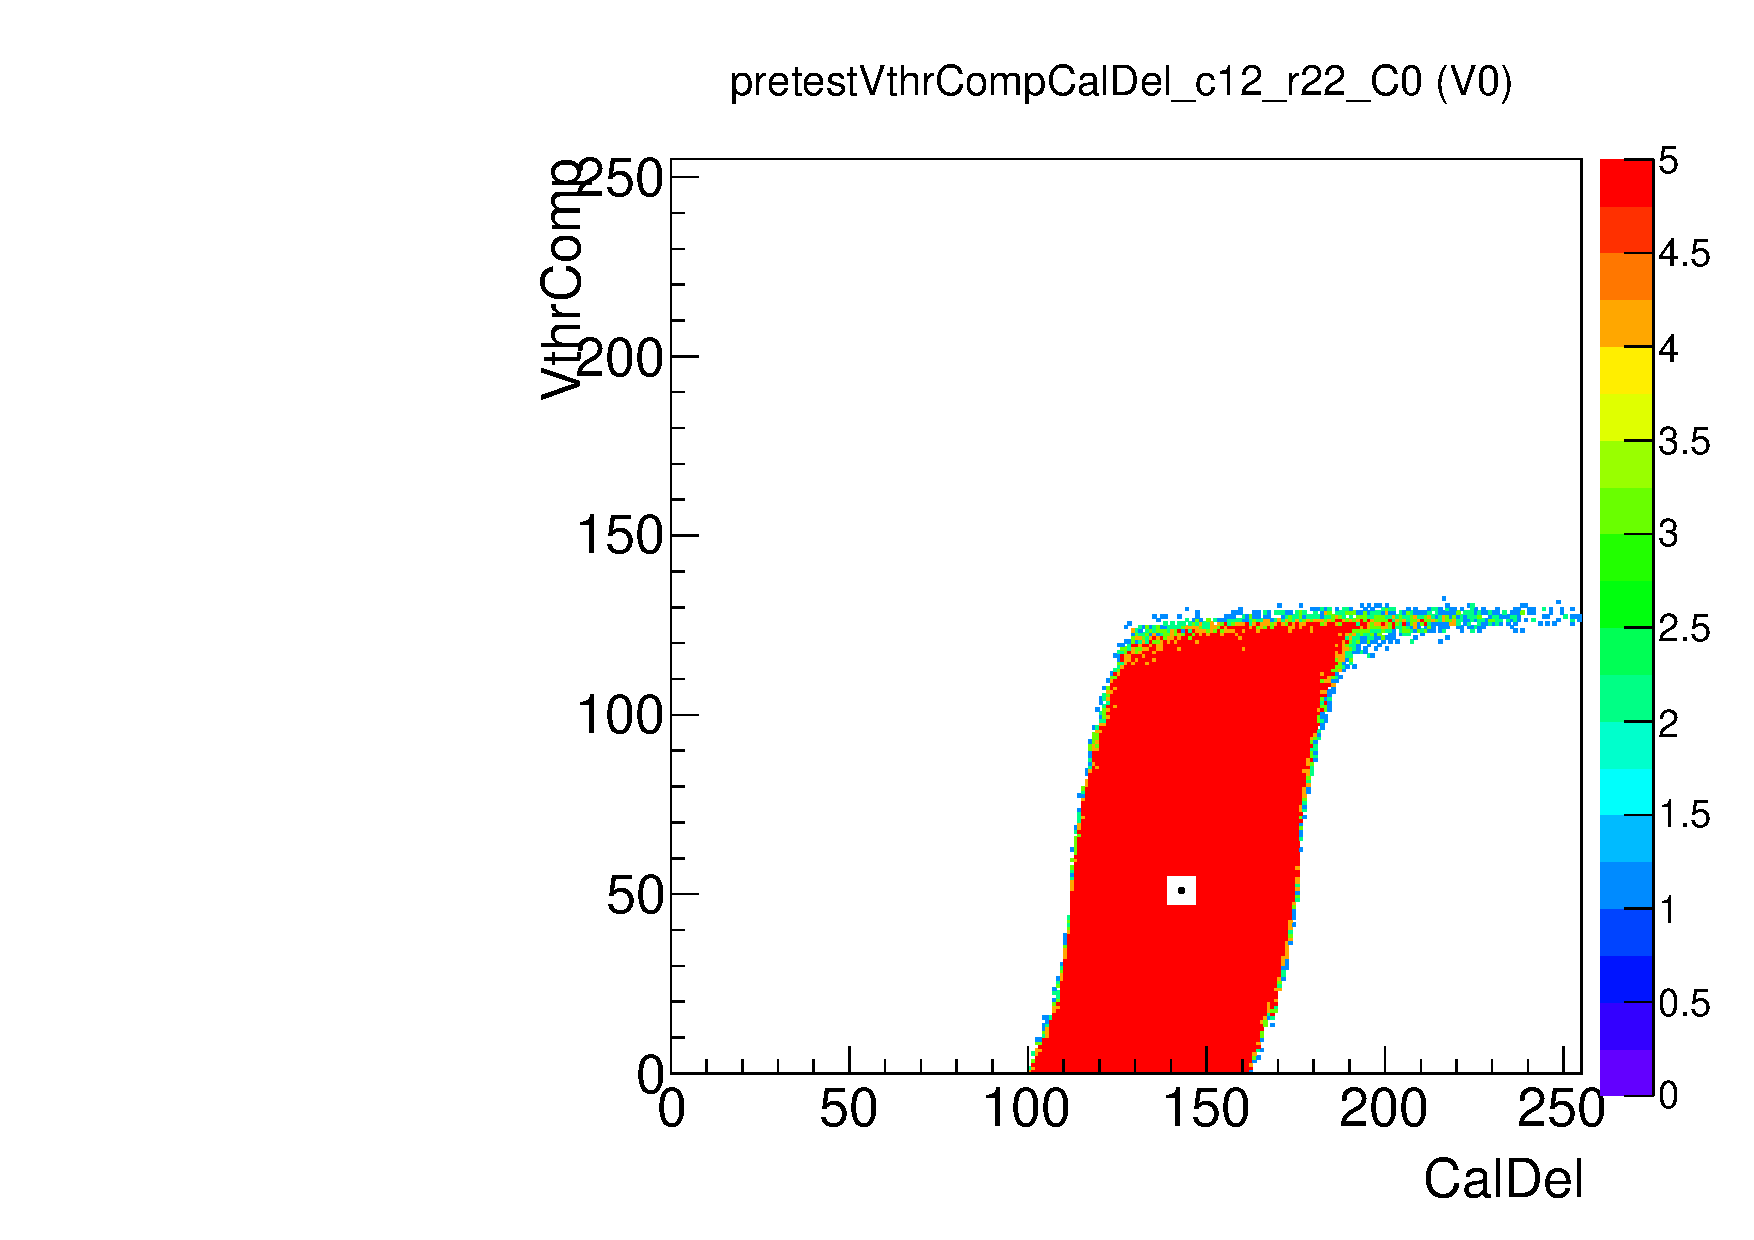
\includegraphics[width=1.0\textwidth]{figures/pretest_pretestVthrCompCalDel_c12_r22.pdf}
  \caption{Tornado plot (efficiency in the \vthrcomp vs. \caldel plane).}
  \label{fig:pretest_pretestVthrCompCalDel_c12_r22}
\end{minipage}
\hspace{0.3cm}
\begin{minipage}{0.45\textwidth}
  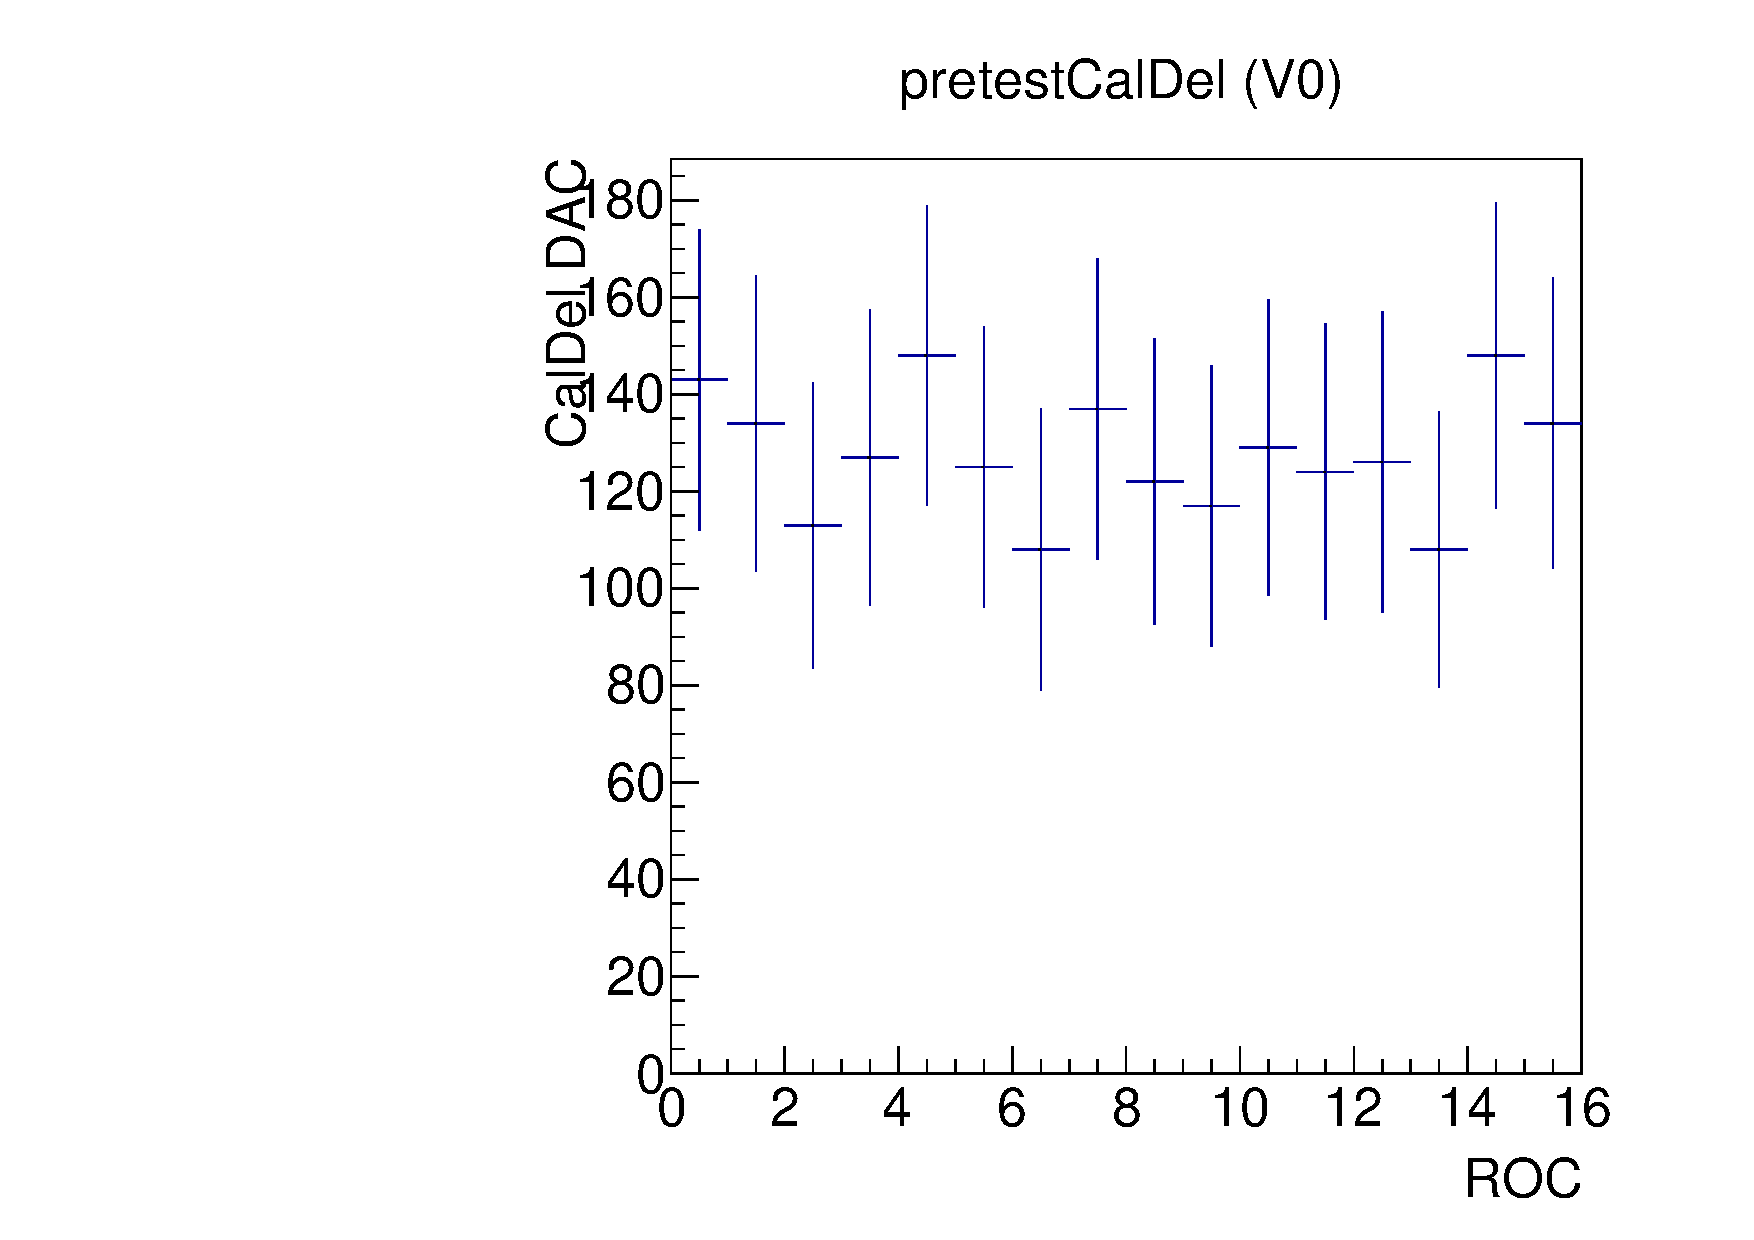
\includegraphics[width=1.0\textwidth]{figures/pretest_pretestCalDel.pdf}
  \caption{The chosen values of \caldel as a function of \roc
    number. The size of the error bars indicates the width of the
    \caldel plateau.}
  \label{fig:pretest_pretestCalDel}
\end{minipage}
\end{figure}


